\documentclass{beamer}
\usetheme{Madrid}
\usepackage{tikz,pgfplots}
\usetikzlibrary{calc}
\usepackage{subfigure}
\newcommand{\norm}[1]{\|#1\|}
\newcommand{\Tube}[6][]%
% [further options], width, iterations, inner color, outer color, path definition
{   \colorlet{InColor}{#4}
	\colorlet{OutColor}{#5}
	\foreach \I in {1,...,#3}
	{   \pgfmathsetlengthmacro{\h}{(\I-1)/#3*#2}
		\pgfmathsetlengthmacro{\r}{sqrt(pow(#2,2)-pow(\h,2))}
		\pgfmathsetmacro{\c}{(\I-0.5)/#3*100}
		\draw[InColor!\c!OutColor, line width=\r, #1] #6;
	}
}

\graphicspath{{figures/}}
\setbeamertemplate{title page}
{
	\begin{centering}
		\begin{beamercolorbox}[sep=8pt,center]{institute}
			\usebeamerfont{institute}\insertinstitute
		\end{beamercolorbox}
		\begin{beamercolorbox}[sep=8pt,center]{title}
			\usebeamerfont{title}\inserttitle\par%
			\ifx\insertsubtitle\@empty%
			\else%
			\vskip0.25em%
			{\usebeamerfont{subtitle}\usebeamercolor[fg]{subtitle}\insertsubtitle\par}%
			\fi%     
		\end{beamercolorbox}%
		\vskip1em\par
		\begin{beamercolorbox}[sep=8pt,center]{date}
			\usebeamerfont{date}\insertdate
		\end{beamercolorbox}%\vskip0.5em
		\begin{beamercolorbox}[sep=8pt,center]{author}
			\usebeamerfont{author}\insertauthor
		\end{beamercolorbox}
	\end{centering}
	%\vfill
}
\makeatother
\institute[IRMA]{Cemosis, IRMA\\ Université de Strasbourg}
% Creates section page in the beginning of each section
\AtBeginSection[]{
	\begin{frame}
		\vfill
		\centering
		\begin{beamercolorbox}[sep=8pt,center,shadow=true,rounded=true]{title}
			\usebeamerfont{title}\insertsectionhead\par%
		\end{beamercolorbox}
		\vfill
	\end{frame}
}
\newcommand\BackgroundPic{%
	\put(0,0){%
		\parbox[b][\paperheight]{\paperwidth}{%
			\vfill
			\centering
			\includegraphics[width=\paperwidth,height=\paperheight,%
			keepaspectratio]{figures/FrontPagePresentation_bottom.pdf}%
			\vfill
}}}


%\title{Micro-swimming framework}
\title{Mathematical and computational frameworks for simulating and optimizing  micro-swimmers}
\author[Berti, Chabannes, Giraldi, Prud'homme]{Luca Berti, Vincent Chabannes, Laetitia Giraldi(Inria), Christophe Prud'homme}
\date{18th May 2021}
\newcommand{\feelpp}{|Feel++|}
\begin{document}
		{\usebackgroundtemplate{\includegraphics[width=\paperwidth]{FrontPagePresentation_bottom.pdf}}
			\begin{frame}[plain]
				\maketitle
			\end{frame}
	}
\begin{frame}
	\frametitle{Some Projects at Cemosis}

	\begin{itemize}
		\item \textbf{IBat} with Synapse-Concept, Febus Ingenierie / Zohra, Vincent, Romain, Yannick 
		\item \textbf{Mordicus} FUI with EDF, Safran, Phimeca, Sorbonne U, ... / Vincent, Romain, Christophe Trphime
		\item \textbf{Eye2brain} with U Paris, U Missouri and Inria / Romain, Vincent, Philippe and Thomas
		\item \textbf{Hifimagnet} with LNCMI / Christophe T, Vincent, Romain V. and Romain 
		\item \textbf{Swimmer} with Inria Sophia / Laetitia, Luca and Vincent
	\end{itemize}
	\begin{alertblock}{}
		Extend, capitalize,  reuse  the work done over the years on Feel++
	\end{alertblock}
\end{frame}
\begin{frame}
	\frametitle{Feel++}

	\begin{itemize}
		\item A large range of numerical methods to solve (parametrized) partial differential
		equations: cG, dG, hdG, crb, \ldots in 1D, 2D and 3D
		\item Powerful interpolation tools in 2D/3D 
		\item  Support for high performance computing up to thousands of cores
		for linear and non-linear problems using  PETSc/SLEPc and
		InHouse solution strategies. (MPI + MT, HPC and Cloud)
		\item Various toolboxes that capitalize our work over the years: CFD, CSM, Heat, Electric, Maxwell and the coupling between them FSI(ALE and LS), heat and fluid, thermoelectric \ldots
		\item New toolbox CFPDEs: arbitrary number of (coupled) linear and non-linear possibly time-dependent PDEs, automatic differentiation, DSL to handle PDE description
	\end{itemize}

\end{frame}
\begin{frame}{Outline}
	\tableofcontents
\end{frame}

	\section{Micro-swimming framework in Feel++}
	\begin{frame}{Mathematical modelling}
		The swimming problem we consider is defined in $\mathcal{F}_t \subseteq\mathbb{R}^d$
		\begin{equation*}
			\left\{
			\begin{aligned}
				-\mu \Delta \textbf{u }+ \nabla p &= f, \quad &\text{in  $\mathcal{F}_t$}\\
				\nabla \cdot \textbf{u} &= 0, \quad &\text{in  $\mathcal{F}_t$}\\
				\textbf{u} &= U+ \Omega \times (x-x^{CM}(t)) + u_d(t) \circ \mathcal{A}_t^{-1}, \quad &\text{on $\partial S_t$ }\\
				m \dot{U} &= F_{ext} -F_{fluid},\\
				J \dot{\Omega} &= M_{ext} -M_{fluid}.
			\end{aligned}
			\right.
			\label{Eq:FEM_Maury0}
		\end{equation*}
	\begin{itemize}
		\item the swimmer $S$ is completely immersed in fluid
		\item $U$ and $\Omega$ are the translational and angular velocities of the body
		\item $u_d$ is the time derivative of the body's displacement
		\item $\mathcal{A}_t$ is the map $\mathcal{F}_0 \to \mathcal{F}_t$, $x \mapsto x + \phi(x)$, where $\phi$ is an extension of the boundary displacement
	\end{itemize}
	\end{frame}
	\begin{frame}{Swimmer motion in the fluid system}
		\begin{equation*}
		\left\{
		\begin{aligned}
		&-\mu \Delta u + \nabla p = 0, \quad &\text{in  $\mathcal{F}_t$},\\
		&\nabla \cdot u = 0, \quad &\text{in  $\mathcal{F}_t$},\\
		&u = U+ \Omega \times (x-x^{CM}) + u_d  \circ \mathcal{A}_t^{-1}, \quad &\text{on  $\partial \mathcal{F}_t \cap \partial S$},\\
		&m \dot{U} = F = F_{ext}-F_{fluid},\\
		&J \dot{\Omega} = M = M_{ext}-M_{fluid}.
		\end{aligned}
		\right.
		\end{equation*}
		Weak formulation $\rightarrow$ test functions ($\tilde{u},\tilde{p},\tilde{U},\tilde{\Omega}$) such that $\tilde{u}=\tilde{U}+\tilde{\Omega}\times (x-x^{CM}) $ on $\partial S$
		\begin{multline*}
		2\mu\int_\mathcal{F} D(u) : D(\tilde{u}) \, dx-\int_{\mathcal{F}} p \nabla\cdot \tilde{u} \, dx + m U \cdot \tilde{U} + 	J \Omega \cdot \tilde{\Omega} \\= F_{ext}\cdot\tilde{U} +M_{ext}\cdot\tilde{\Omega}.
		\label{Eq:Compacted}
		\end{multline*}
		\begin{thebibliography}{9}	\setbeamertemplate{bibliography item}[article]\bibitem{Maury1999} \tiny
		B. Maury, \textit{Direct Simulations of 2D Fluid-Particle Flows in Biperiodic Domains}. Journal of Computational Physics, 156, 1999.
		\end{thebibliography}
		\end{frame}
		\begin{frame}{Numerical techniques}
			\begin{itemize}
				\item spatial discretization $\to$ conforming Lagrange finite elements
				\item moving fluid domain $\to$ Arbitrary-Lagrangian-Eulerian frame
				\item rigid body velocity $\to$ constrain fluid velocity $\textbf{u}$ to the subspace 
				\[
					V_{R} = \{\textbf{u} \in [H^1(\mathcal{F})]^d\, |\, \textbf{u}|_{\partial S}  = U+\Omega\times (x-x^{CM}) \text{ for $U,\Omega \in \mathbb{R}^d$}\}
				\]
				\item mesh adaptation $\to$ harmonic extension and remeshing
			\end{itemize}
		\end{frame}
		\begin{frame}{Algebraic form (I)}
			We need to enforce the condition $\mathbf{\tilde{u}=\tilde{U}+\tilde{\Omega}\times (x-x^{CM})} $ \textbf{on $\mathbf{\partial S}$ }on the test functions.
			\begin{itemize}
			\item We build the system matrix $A$. No coupling for the moment is enforced between fluid and swimmer.
			\begin{equation*}
			A = 
			\begin{bmatrix}
			A_{II} & A_{I\Gamma} & 0 & 0 & B_{I}^T  \\
			A_{\Gamma I} & A_{\Gamma \Gamma}  & 0 & 0 & B_{\Gamma}^T\\
			0 & 0 & T & 0 & 0 \\
			0 & 0 & 0& R & 0\\
			B_I & B_\Gamma & 0 & 0 & 0   \\
			\end{bmatrix}
			\end{equation*}
			\item We build a coupling matrix $\mathcal{P}$ such that $(u_I,u_{\partial S},U,\Omega,p)^T = \mathcal{P} (u_I,u_{\partial S},U,\Omega,p)^T$
			\begin{equation*}
			\mathcal{P} =
			\begin{bmatrix}
			I & 0 & 0 & 0 & 0\\
			0 &  0 & \tilde{P}_U & \tilde{P}_\Omega& 0\\
			0 & 0 & I & 0 & 0\\
			0 & 0 & 0 & I & 0\\
			0 & 0& 0& 0& I
			\end{bmatrix}
			\end{equation*}
			\end{itemize}
		\end{frame}
		\begin{frame}{Algebraic form (II)}
			\begin{multline*}
			\mathcal{P}^T \begin{bmatrix}
			A_{II} & A_{I\Gamma} & 0 & 0 & B_{I}^T  \\
			A_{\Gamma I} & A_{\Gamma \Gamma}  & 0 & 0 & B_{\Gamma}^T\\
			0 & 0 & T & 0 & 0 \\
			0 & 0 & 0& R & 0\\
			B_I & B_\Gamma & 0 & 0 & 0   \\
			\end{bmatrix} \mathcal{P} 
			\\= 
			\begin{bmatrix}
			A_{II} & \textbf{0} & A_{I\Gamma}\tilde{P}_U   & A_{I\Gamma}  \tilde{P}_\Omega  & B_{I}^T  \\
			\textbf{0} & \textbf{\textcolor{red}{I}} & \textbf{0} & \textbf{0} & \textbf{0} \\
			\tilde{P}_U^T A_{\Gamma I} & \textbf{0} & \tilde{P}_U ^T A_{\Gamma \Gamma} \tilde{P}_U  + T   & \tilde{P}_U ^T A_{\Gamma \Gamma} \tilde{P}_\Omega & \tilde{P}_U^TB_{\Gamma}^T\\
			\tilde{P}_\Omega^T A_{\Gamma I} & \textbf{0} & \tilde{P}_\Omega ^T A_{\Gamma \Gamma} \tilde{P}_U & \tilde{P}_\Omega ^T A_{\Gamma \Gamma} \tilde{P}_\Omega  + R& \tilde{P}_\Omega^TB_{\Gamma}^T\\
			B_I & \textbf{0}  & B_\Gamma\tilde{P}_U &  B_\Gamma\tilde{P}_\Omega & 0   \\
			\end{bmatrix}.
			\end{multline*}
	\end{frame}

\begin{frame}
	\frametitle{Comments on the resulting system}

	Solve 
	\begin{equation}
		\mathcal{P}^T A  
		\begin{bmatrix}
			u_I\\
			u_{\partial S} \\
			U \\
			\Omega\\
			p
		\end{bmatrix} 
		=
		\mathcal{P}^T A \mathcal{P} 
		\begin{bmatrix}
			u_I\\
			u_{\partial S} \\
			U \\
			\Omega\\
			p
		\end{bmatrix} 
		= \mathcal{P}^T
		\begin{bmatrix}
			F_I\\
			0 \\
			F_\mathrm{ext} \\
			M_\mathrm{ext}\\
			0
		\end{bmatrix} 
		- \mathcal{P}^T A
		\begin{bmatrix}
		 0\\
		 u_d \circ \mathcal{A}_t^{-1}\\
		 0\\
		 0\\
		 0\\
		\end{bmatrix} 
	\end{equation}
	\begin{itemize}
		\item Requires efficient implementation of $\mathcal{P}^T A \mathcal{P}$ specially in parallel. The matrix is actually assembled.
		\item Use a block preconditioner of type PCD or PMM depending on the regime by grouping together velocity unknowns.
		\item Velocity blocks are split further between fluid velocity and rigid body velocities and use an (inexact)  gauss seidel  preconditioner
		\item The PETSc support in feelpp enables all these steps.
		\item Now the swimmer may have  large displacements, remeshing is necessary
	\end{itemize}

\end{frame}

	\section{Mesh adaptation}
	\begin{frame}{Remeshing in Feel++ using (Par)MMG}
		\begin{columns}
			\begin{column}{0.49\textwidth}
				\includegraphics[width=\linewidth]{2d_remeshing.png}
			\end{column}
			\begin{column}{0.49\textwidth}
					\includegraphics[width=\linewidth]{DRIVEN_CAVITY.png}
			\end{column}
		\end{columns}
		\begin{columns}
			\begin{column}{0.5\textwidth}
					\includegraphics[width=\linewidth]{3D_SLIDING.png}
			\end{column}
			\begin{column}{0.49\textwidth}
				\begin{itemize}
					\item Edge split
					\item Edge collapse
					\item Edge swap
					\item Node relocation
					\item Local size function $h$
					\item lots of ways to control the metric 
				\end{itemize}
			\end{column}
		\end{columns}
		\begin{thebibliography}{9}	\setbeamertemplate{bibliography item}[article]\bibitem{Dapogny2014}{\tiny \textit{Three-dimensional adaptive domain remeshing, implicit domain meshing, and applications to free and moving boundary problems} - C. Dapogny, C. Dobrzynski and P. Frey - April 1, 2014 - JCP
				
			}
		\end{thebibliography}
	\end{frame}
\begin{frame}
	\frametitle{Parallel remeshing}
	\begin{columns}
		\begin{column}{.5\linewidth}
			\includegraphics[width=.7\linewidth]{par-mesh-n6-1.png}\\
			\includegraphics[width=.7\linewidth]{par-remesh-n6-1.png}
		\end{column}
		\begin{column}{.5\linewidth}
			\begin{itemize}
				\item Parallel remeshing is a challenge and MMG provides an initial version last Autumn
				\item Iterative strategy: remesh in subdomains while keeping interprocess faces fixed and iterate after repartitioning.
			\end{itemize}
		\end{column}
	\end{columns}

	
	

\end{frame}

\begin{frame}{Remeshing metric}
	\begin{equation*}
		h_{new}(x) = 
		\left\{
		\begin{aligned}
			h_{avg} &\quad \text{if $dist(x,\partial S_t) \le nh_{avg} $}\\
			h_{avg}*c_\mathrm{far}	 &\quad \text{if $dist(x,\partial S_t) > nh_{avg} $}
		\end{aligned}
		\right.
	\end{equation*}
	where 
	\begin{itemize}
		\item $h_{new}(x)$ is the mesh size passed to MMG, other recipes can be applied depending on context
		\item $h_{avg}$ is the average mesh size of the swimmer
		\item $dist$ is the distance to the swimmer computed using a (parallel) fast marching algorithm
		\item $nh_{avg}$ provides a distance threshold away from the swimmer
		\item $c_{\mathrm{far}}$ is a coefficient greater than 1 to get larger elements far away
		\item Gradation mechanism of MMG smoothes out the edge length increase
		%\item $\alpha$ is a prescribed constant
		%\item $h$ is the characteristic size of the previous mesh
	\end{itemize}
\end{frame}
	\begin{frame}{Parent-son relationship for meshes}
		To evaluate expressions $u_d \circ \mathcal{A}_t^{-1}$ in the swimmer's reference frame, the initial reference mesh must be stored.
		\begin{itemize}
			\item define the elements/faces that remain unvaried across remeshing
			\item create a bijective correspondence between these elements/faces in the two meshes
			\item evaluation of  expressions is now realized on the parent mesh
			\item there is no localization at all necessary in the interpolation process.
			\item This is implemented thanks to the required element feature of MMG with a twist to build the relation.
		\end{itemize}
	\end{frame}
	\begin{frame}{Remeshing and interpolation}		
		Using ALE to handle moving domains is possible under the condition that movements are not too large.
		\begin{alertblock}{Available mesh quality indices}
			\begin{equation*}
				q_{2D} = \frac{4A^2}{|e_1||e_2||e_3|2p}, \, q_{2D-BX} = \frac{4\sqrt{3}A}{|e_1|^2+|e_2|^2+|e_3|^2}, \, q_{3D} = \frac{2^3 3^8 \sqrt{3}V^4}{(\sum_{i=1}^{4} A_1^2)^3}
			\end{equation*}	
		\end{alertblock}
		We constrain:
		\begin{itemize}
			\item Interfaces, that must be kept,
			\item Interface discretization, that should be remain unvaried as well (in order to maintain all the properties linked to areas and volumes of the enclosed region),
			\end{itemize}
			We interpolate the solution from the old to the new mesh, in order to restart computations.
	\end{frame}
\begin{frame}{Mesh adaptation for swimming simulations}
	We individuated three remeshing procedures that corresponded to different needs of our model swimmers:
	\begin{itemize}
		\only<1>{\item Initial mesh size distribution $\neq$ Desired mesh size distribution
		\includegraphics[width=0.45\linewidth]{gait-2.png}
		\includegraphics[width=0.45\linewidth]{nature-remesh-1.png}
		\begin{itemize}
			\item Define the mesh size distribution in the fluid
			\item Remesh by keeping fixed the elements in the swimmer
	\end{itemize}}
		
		\only<2>{\item Reference swimmer configuration $\neq$ Swimmer configuration at $t=0$
			\includegraphics[width=0.45\linewidth]{gait-2.png}
		\includegraphics[width=0.45\linewidth]{gait-3.png}
	\begin{itemize}
		\item Define the displacement in the reference configuration and fraction it in sub-steps
		\item Alternate harmonic extensions and remeshing steps until the $t=0$ position is reached
\end{itemize}}
		
		\only<3>{\item Reaching the desired configuration by sub-steps (3d and 2d)
			\includegraphics[width=0.45\linewidth]{gait-6.png}
			\includegraphics[width=0.45\linewidth]{gait-7.png}
			\begin{itemize}
				\item Given the displacement $\eta_{n+1}$, fraction it in sub-steps
				\item Alternate harmonic extensions and remeshing steps until the  position at $t=t_{n+1}$ is reached
			\end{itemize}
		}
	\end{itemize}
\end{frame}
	\section{Examples of swimmers}
	\begin{frame}{Articulated swimmers}
		\begin{figure}
			\centering
			\resizebox{0.8\textwidth}{!}{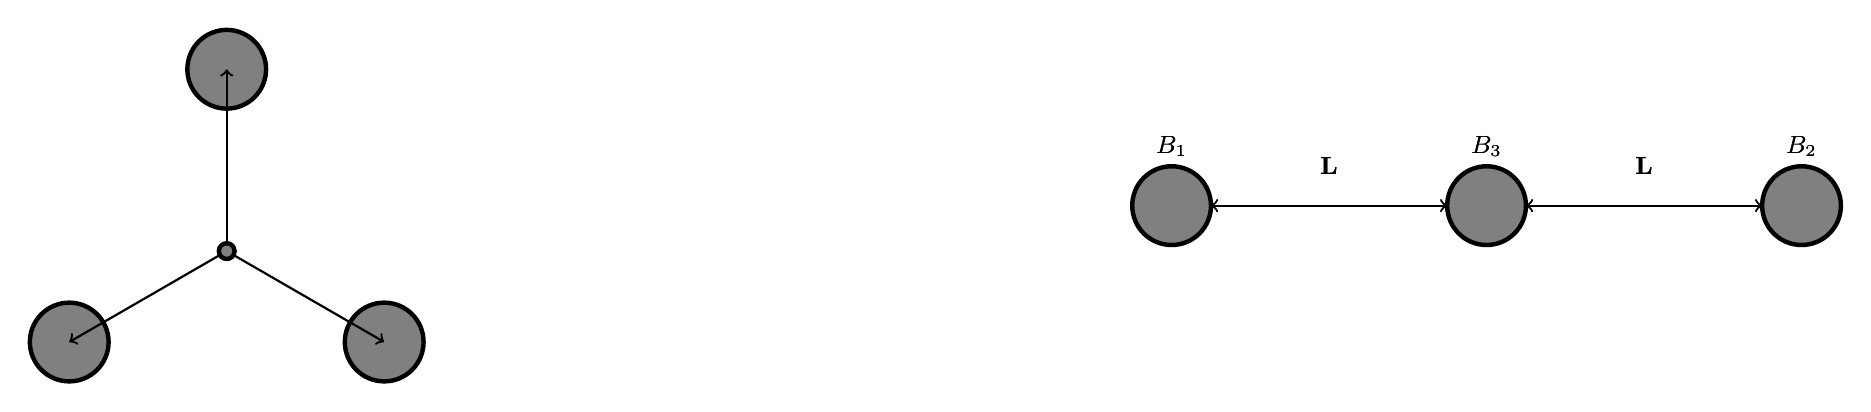
\begin{tikzpicture}
					\draw[ultra thick,, fill=gray]  (-4,0) ellipse (0.5cm and 0.5cm);
					\draw[ultra thick,, fill=gray]  (0,0) ellipse (0.5cm and 0.5cm);
					\draw[ultra thick,, fill=gray]  (4,0) ellipse (0.5cm and 0.5cm);
					\draw[thick,<->] (-3.5,0) -- (-0.5,0);
					\draw[thick,<->] (3.5,0) -- (0.5,0);
					\node at (-2,0.5) {\small\bf L};
					\node at (2,0.5)  {\small\bf L};
					\node at (-4,0.75) {\small\bf $B_1$};
					\node at (4,0.75) {\small\bf $B_2$};
					\node at (0,0.75) {\small\bf $B_3$};
					
					\draw[ultra thick,, fill=gray]  (-18,-4*1.732/4) ellipse (0.5cm and 0.5cm);
					\draw[ultra thick,, fill=gray]  (-16,4*1.732/4) ellipse (0.5cm and 0.5cm);
					\draw[ultra thick,, fill=gray]  (-14,-4*1.732/4) ellipse (0.5cm and 0.5cm);
					\draw[thick,<->] (-18,-4*1.732/4) -- (-16,-1.732+2/1.732);
					\draw[thick,<->] (-16,4*1.732/4) -- (-16,-1.732+2/1.732);
					\draw[thick,<->] (-14,-4*1.732/4) -- (-16,-1.732+2/1.732);
					\draw[ultra thick,, fill=gray]  (-16,-1.732+2/1.732) ellipse (0.1cm and 0.1cm);
					\node at (-2,0.5) {\small\bf L};
					\node at (2,0.5)  {\small\bf L};
					\node at (-4,0.75) {\small\bf $B_1$};
					\node at (4,0.75) {\small\bf $B_2$};
					\node at (0,0.75) {\small\bf $B_3$};
				\end{tikzpicture}
			}
			\caption{Example of articulated swimmers with translational constraints}
		\end{figure}
	\vspace{-0.5cm}
		\begin{itemize}
			\item Analytical computations and benchmarking
			\item Slight modification of independent rigid bodies formulation
		\end{itemize}
		Procedure:
		\begin{itemize}
			\item Identify $B_n$ as the reference body
			\item $\textbf{U}_i$ of all the other bodies $B_i$, $i=1\ldots n-1$, are expressed as functions of $\textbf{U}_n$ via constraints of the form 
			\begin{equation*}
				\textbf{U}_i =\textbf{U}_n+\textbf{W}_{in}(t), \quad  i=1\ldots n-1,
				\label{Eq:constraints}
			\end{equation*}
		\end{itemize}
		where $\textbf{W}_{in}(t)$ represents the relative velocity between $B_i$ and $B_n$.
	\end{frame}
\begin{frame}{Translational constraints - Lagrange multipliers}
	Lagrange multipliers:
	\begin{equation*}
		\dot{\textbf{U}}_i \cdot \tilde{\textbf{U}}_i +\alpha_i \cdot \tilde{\textbf{U}}_i= 0 \quad i=1\ldots n-1,
		\label{Eq:Trans2}
	\end{equation*}
	\begin{equation*}
		\dot{\textbf{U}}_n \cdot \tilde{\textbf{U}}_n -\sum_{i=1}^{n-1}\alpha_i \cdot \tilde{\textbf{U}}_n= 0%- \int_{\partial B_n} (-pI + 2\mu D(u)) \vec{n} \cdot \tilde{\textbf{U}}_n\, dS, 
		\label{Eq:Trans3}
	\end{equation*}
	\begin{equation*}
		{\alpha_i \cdot(\textbf{U}_i-\textbf{U}_n} )= \alpha_i \cdot \textbf{W}_{in}, \quad i=1\ldots n-1.
		\label{Eq:Multipliers}
	\end{equation*}
	The addition of Lagrange multipliers entails further constraints on the space $V_R$, which are reflected in the coupling operator between $\textbf{u}$ and $\textbf{U}_i$.
\end{frame}
	\begin{frame}{Three sphere swimmer}
		It is made of three sphere of radius $R$. The lateral spheres are separated from the central one by a distance of $L$. 
		
		This object swims by retracting and elongating its arms in a non-reciprocal fashion.
		
		\begin{figure}
			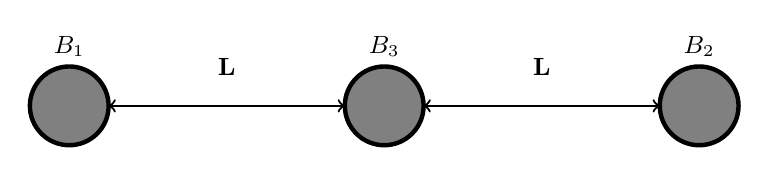
\begin{tikzpicture}
				\draw[ultra thick,, fill=gray]  (-4,0) ellipse (0.5cm and 0.5cm);
				\draw[ultra thick,, fill=gray]  (0,0) ellipse (0.5cm and 0.5cm);
				\draw[ultra thick,, fill=gray]  (4,0) ellipse (0.5cm and 0.5cm);
				\draw[thick,<->] (-3.5,0) -- (-0.5,0);
				\draw[thick,<->] (3.5,0) -- (0.5,0);
				\node at (-2,0.5) {\small\bf L};
				\node at (2,0.5)  {\small\bf L};
				\node at (-4,0.75) {\small\bf $B_1$};
				\node at (4,0.75) {\small\bf $B_2$};
				\node at (0,0.75) {\small\bf $B_3$};
			\end{tikzpicture}
		\end{figure}
		Analytical results describing its motion are available.
		\footnote{\tiny A. NAJAFI AND R. GOLESTANIAN, Simple swimmer at low reynolds number: Three linked spheres, Physical
		review. E, Statistical, nonlinear, and soft matter physics, 69 (2004)}
	\end{frame}
	\begin{frame}{Results}
	\begin{figure}
		\centering
		\resizebox{0.3\textwidth}{!}{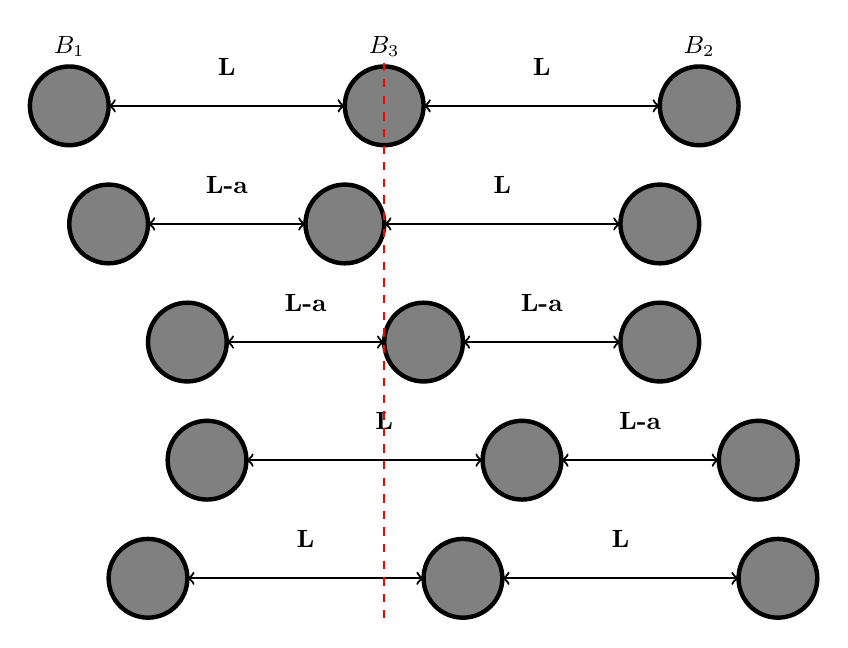
\begin{tikzpicture}
				\draw[ultra thick,, fill=gray]  (-4,0) ellipse (0.5cm and 0.5cm);
				\draw[ultra thick,, fill=gray]  (0,0) ellipse (0.5cm and 0.5cm);
				\draw[ultra thick,, fill=gray]  (4,0) ellipse (0.5cm and 0.5cm);
				\draw[thick,<->] (-3.5,0) -- (-0.5,0);
				\draw[thick,<->] (3.5,0) -- (0.5,0);
				\node at (-2,0.5) {\small\bf L};
				\node at (2,0.5)  {\small\bf L};
				\node at (-4,0.75) {\small\bf $B_1$};
				\node at (4,0.75) {\small\bf $B_2$};
				\node at (0,0.75) {\small\bf $B_3$};
				
				\draw[ultra thick,, fill=gray]  (-3.5,-1.5) ellipse (0.5cm and 0.5cm);
				\draw[ultra thick,, fill=gray]  (-0.5,-1.5) ellipse (0.5cm and 0.5cm);
				\draw[ultra thick,, fill=gray]  (3.5,-1.5) ellipse (0.5cm and 0.5cm);
				\draw[thick,<->] (-3,-1.5) -- (-1,-1.5);
				\draw[thick,<->] (0,-1.5) -- (3,-1.5);
				\node at (-2,-1) {\small\bf L-\textbf{a}};
				\node at (1.5,-1)  {\small\bf L};
				
				\draw[ultra thick,, fill=gray]  (-2.5,-3) ellipse (0.5cm and 0.5cm);
				\draw[ultra thick,, fill=gray]  (0.5,-3) ellipse (0.5cm and 0.5cm);
				\draw[ultra thick,, fill=gray]  (3.5,-3) ellipse (0.5cm and 0.5cm);
				\draw[thick,<->] (-2,-3) -- (0,-3);
				\draw[thick,<->] (3,-3) -- (1,-3);
				\node at (-1,-2.5) {\small\bf L-a};
				\node at (2,-2.5)  {\small\bf L-a};
				
				\draw[ultra thick,, fill=gray]  (-2.25,-4.5) ellipse (0.5cm and 0.5cm);
				\draw[ultra thick,, fill=gray]  (1.75,-4.5) ellipse (0.5cm and 0.5cm);
				\draw[ultra thick,, fill=gray]  (4.75,-4.5) ellipse (0.5cm and 0.5cm);
				\draw[thick,<->] (-1.75,-4.5) -- (1.25,-4.5);
				\draw[thick,<->] (4.25,-4.5) -- (2.25,-4.5);
				\node at (0,-4) {\small\bf L};
				\node at (3.25,-4)  {\small\bf L-a};
				
				\draw[ultra thick,, fill=gray]  (-3,-6) ellipse (0.5cm and 0.5cm);
				\draw[ultra thick,, fill=gray]  (1,-6) ellipse (0.5cm and 0.5cm);
				\draw[ultra thick,, fill=gray]  (5,-6) ellipse (0.5cm and 0.5cm);
				\draw[thick,<->] (-2.5,-6) -- (0.5,-6);
				\draw[thick,<->] (4.5,-6) -- (1.5,-6);
				\node at (-1,-5.5) {\small\bf L};
				\node at (3,-5.5)  {\small\bf L};
				
				\draw[dashed,red, thick] (0,0.55) -- (0,-6.5);
			\end{tikzpicture}
		}
		\includegraphics[width=0.3\textwidth]{W_cl.png}
		\includegraphics[width=0.3\textwidth]{CM_evolution_1.png}
		\caption{Three-sphere swimmer and its swimming gait.}
		
		\label{Fig:results}
		\begin{center}
			\includegraphics[width=0.5\linewidth]{Threespheres.png}
		\end{center}
	\end{figure}
\footnote{\tiny Luca Berti, Vincent Chabannes, Laetitia Giraldi, Christophe Prud'Homme. Modeling and finite element simulation of multi-sphere swimmers. 2020.}

	\end{frame}
%	\begin{frame}{Imposed motion of the centreline}
%		\begin{itemize}
%			\item Analytical motion (easy functional form)
%			
%			(put sperm 2d)
%			\item Centreline motion from ODEs 
%			
%			(put example of Nature 2d and 3d)			
%		\end{itemize}
%	\end{frame}
%\begin{frame}{Analytical motion - results}
%	\begin{itemize}
%	\item Different beating amplitudes
%		\item Different channel heights
%		\item Different head sizes
%	\end{itemize}
%	\begin{figure}
%	\centering
%		\begin{tikzpicture} 
%%			\begin{axis}%[xlabel={$A_{max} \,\,[\mu m]$}, ylabel={$V \,\,[\mu m /s]$},xmajorgrids,ymajorgrids,
%%%				scatter/classes={%
%%%					a={mark=square*,blue},%
%%%					b={mark=o,black},
%%%					c={mark=triangle*,red},
%%%					d={mark=square*,green}},scatter, mark=*,
%%%				scatter src=explicit symbolic,legend entries={
%%%					h=7.5$\mu m$,
%%%					h=15$\mu m$,
%%%					h=7.5$\mu m$ \cite{RazaviAhmadi2015},
%%%					h=15$\mu m$ \cite{RazaviAhmadi2015}
%%%				},
%%%				legend pos=outer north east]
%%				\addplot[scatter,line width=1pt,blue]
%%				table[meta = class] {
%%					x        y   class
%%					1 1.37 a
%%					2 5.13 a 
%%					3 9.7 a
%%				};
%%%				\addplot[scatter,line width=1pt,red]
%%%				table[meta = class] {
%%%					x        y   class
%%%					1 1.6 c
%%%					2 5.8 c 
%%%					3 10 c
%%%				};
%%%			\end{axis}
%	\end{tikzpicture}
%	\end{figure}
%\end{frame}
\begin{frame}{Centreline motion from ODEs}
	\begin{itemize}
		\item Position vector $\textbf{r}$
		\item Cosserat reference frame $\{\textbf{e}_1,\textbf{e}_2,\textbf{e}_3\}$
		\item  arclength coordinate $l$
		\item torsion parameter $\tau_f$
		\item curvature function $\kappa_f$
	\end{itemize}
	\begin{columns}
		\begin{column}{0.6\textwidth}
				\begin{equation*}
				\left\{
				\begin{aligned}
					\frac{d\textbf{r}}{dl}&=-\textbf{e}_3,\\
					\frac{d\textbf{e}_1}{dl}&=-\kappa_f \textbf{e}_3+\tau_f \textbf{e}_2, \\
					\frac{d\textbf{e}_2}{dl}&=-\tau_f \textbf{e}_1, \\
					\frac{d\textbf{e}_3}{dl}&=\kappa_f \textbf{e}_1.
				\end{aligned}
				\right.
				\label{Eq: Jikeli}
			\end{equation*}
		\end{column}
	\begin{column}{0.3\textwidth}
		\begin{figure}
			\resizebox{0.8\linewidth}{!}{\begin{tikzpicture}[>=stealth,pics/tang/.style={code={
						\draw[white,->] (0,0) coordinate (M)-- (2,0) coordinate (v) node[pos=1.1]{$\vec v$}; 
				}}]
				\draw[red,semithick] (0.2,3.6) to[bend left] 
				pic[pos=0.4,sloped]{tang} (3.8,1);
				\draw[green!60!black,->] (M) -- ($(M)!1cm!(0,-1)$) coordinate[label={left:{$\textbf{e}_1$}}] (n);
				\path ($ (n)!1cm!-90:(M) $) coordinate (aux1) (M)++(0,-1) coordinate (aux2)
				(intersection of n--aux1 and M--aux2) coordinate (a)
				($(M)!(a)!(v)$) coordinate (tau);
				\draw[black,->] (-1,-1)--(M) node[pos=0.5,above] {$\textbf{r}$};
				\draw[brown,->] (M)   -- (tau)node[pos=1.2,above]{$\textbf{e}_3$};    
				\draw[blue,->] (M)   -- (M)node[pos=1.2,above]{$\textbf{e}_2$};    
			\end{tikzpicture}}
		\end{figure}
	\end{column}
	\end{columns}
\end{frame}
\begin{frame}{Create the 2D/3D mesh from the centerline}		
		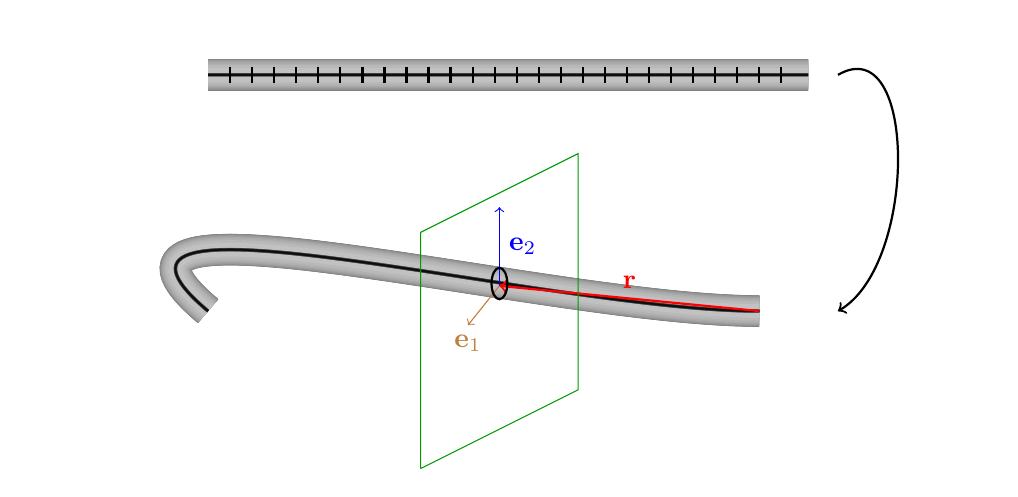
\begin{tikzpicture}
			\Tube{4mm}{10}{gray!45}{black!55}
			{(-7,3) to[out=0,in=0] (0,3)}
			\Tube{0.5mm}{10} {black!100}{black!0}
			{(-7,3) to[out=0,in=0] (0,3)}
			\draw[thick,->] (1,3) to [out=30,in=30] (1,0);
\foreach \i in {1,...,26}
{\draw[thick] (-7+\i*7/25,3.1) -- (-7+\i*7/25,2.9); }
			\Tube{4mm}{10}{gray!45}{black!55}
			{(-7,0) to[out=140,in=180] (0,0)}
			\Tube{0.5mm}{10} {black!100}{black!0}
			{(-7,0) to[out=140,in=180] (0,0)}
			\draw[red,thick,->] (0,0) -- (-3.3,0.32) node[pos=0.5,above] {$\textbf{r}$};
			\draw[green!60!black]  (-4.3,-2) -- (-2.3,-1) -- (-2.3,2) --(-4.3,1) --(-4.3,-2) ;
			\draw[blue,->] (-3.3,0.32)   -- (-3.3,1.32)node[pos=0.5,right]{$\textbf{e}_2$};    
			\draw[brown,->] (-3.3,0.32)   -- (-3.7,-0.18)node[pos=1.0,below]{$\textbf{e}_1$};    
			\draw[black,thick] (-3.3,0.35) ellipse (1mm and 2mm);
		\end{tikzpicture}
	\begin{figure}
		\begin{itemize}
			\item parallel transported frame (to avoid rotating sections along the tail)
			\item linear interpolation of  position between nodes of the 1D model
			\item extend the 1D motion to the orthogonal section via $\textcolor{brown}{\textbf{e}_1},\textcolor{blue}{\textbf{e}_2}$
		\end{itemize}
	\end{figure}
\end{frame}
\begin{frame}{Position Vs Velocity formulation}
	Via automatic differentiation, we can obtain \[\frac{d\textbf{r}}{dt}, \frac{d\textbf{e}_1}{dt},\frac{d\textbf{e}_2,}{dt}\frac{d \textbf{e}_3}{dt}.\] 
	We can recover $\textbf{r},\textbf{e}_1,\textbf{e}_2,\textbf{e}_3$ by time integration
\begin{figure}
	\caption[caption]{ Left: Implicit Euler scheme (blue) and position (red).
		Right: Runge-Kutta 4 scheme (green) vs Implicit Euler scheme (blue).}
	\includegraphics[width=0.45\linewidth]{gait-5.png}
	\includegraphics[width=0.45\linewidth]{gait-4.png}
\end{figure}
\end{frame}
\begin{frame}
	\frametitle{Spermatozoon 2D and 3D}

	\begin{itemize}
		\item Analytical displacement velocity 2D and 3D
		\item various parameters (like amplitude) allowing to test the robusteness of the framework and benchmarking with Comsol possible in 2D
	\end{itemize}

\end{frame}
	\section{Perspectives}
	\begin{frame}{Fluid-solid interaction}
		\begin{itemize}
			\item Couple a moving hyper-elastic swimmer to the fluid (externally powered)
			\item Propose two active-elasticity models to be used in the framework (M1 projects)
			
			Visible elastic effects $\to$ passive and active components
			\begin{equation*}
				\begin{aligned}
					\Sigma_p &= \Sigma_{visible}-\Sigma_a e_a\otimes e_a \qquad &\text{(Additive model)}\\
					F_p &= F_{visible}F_a^{-1} \qquad &\text{(Multiplicative model)}
				\end{aligned}
			\end{equation*}
		\item Managing mesh adaptation and motion with Lagrangian description of elasticity
		\item Add rigid-body velocity in the FSI coupling conditions
		\end{itemize}
	\end{frame}
	\begin{frame}{Learning to swim}
		Learn optimal swimming strategies for multi-sphere swimmers via Q-learning (M2 stage).
		\begin{figure}
			\centering
			\includegraphics[width=0.5\linewidth]{figures/Multisphere.png}
		\end{figure}
	\begin{itemize}
		\item steady fluid
		\item background flow
		\item next to boundaries
	\end{itemize}
	\end{frame}

\end{document}